% \subsection{水资源治理变化过程}\label{ch4:sec:process}

\begin{figure*}[ht!]
	\centering
	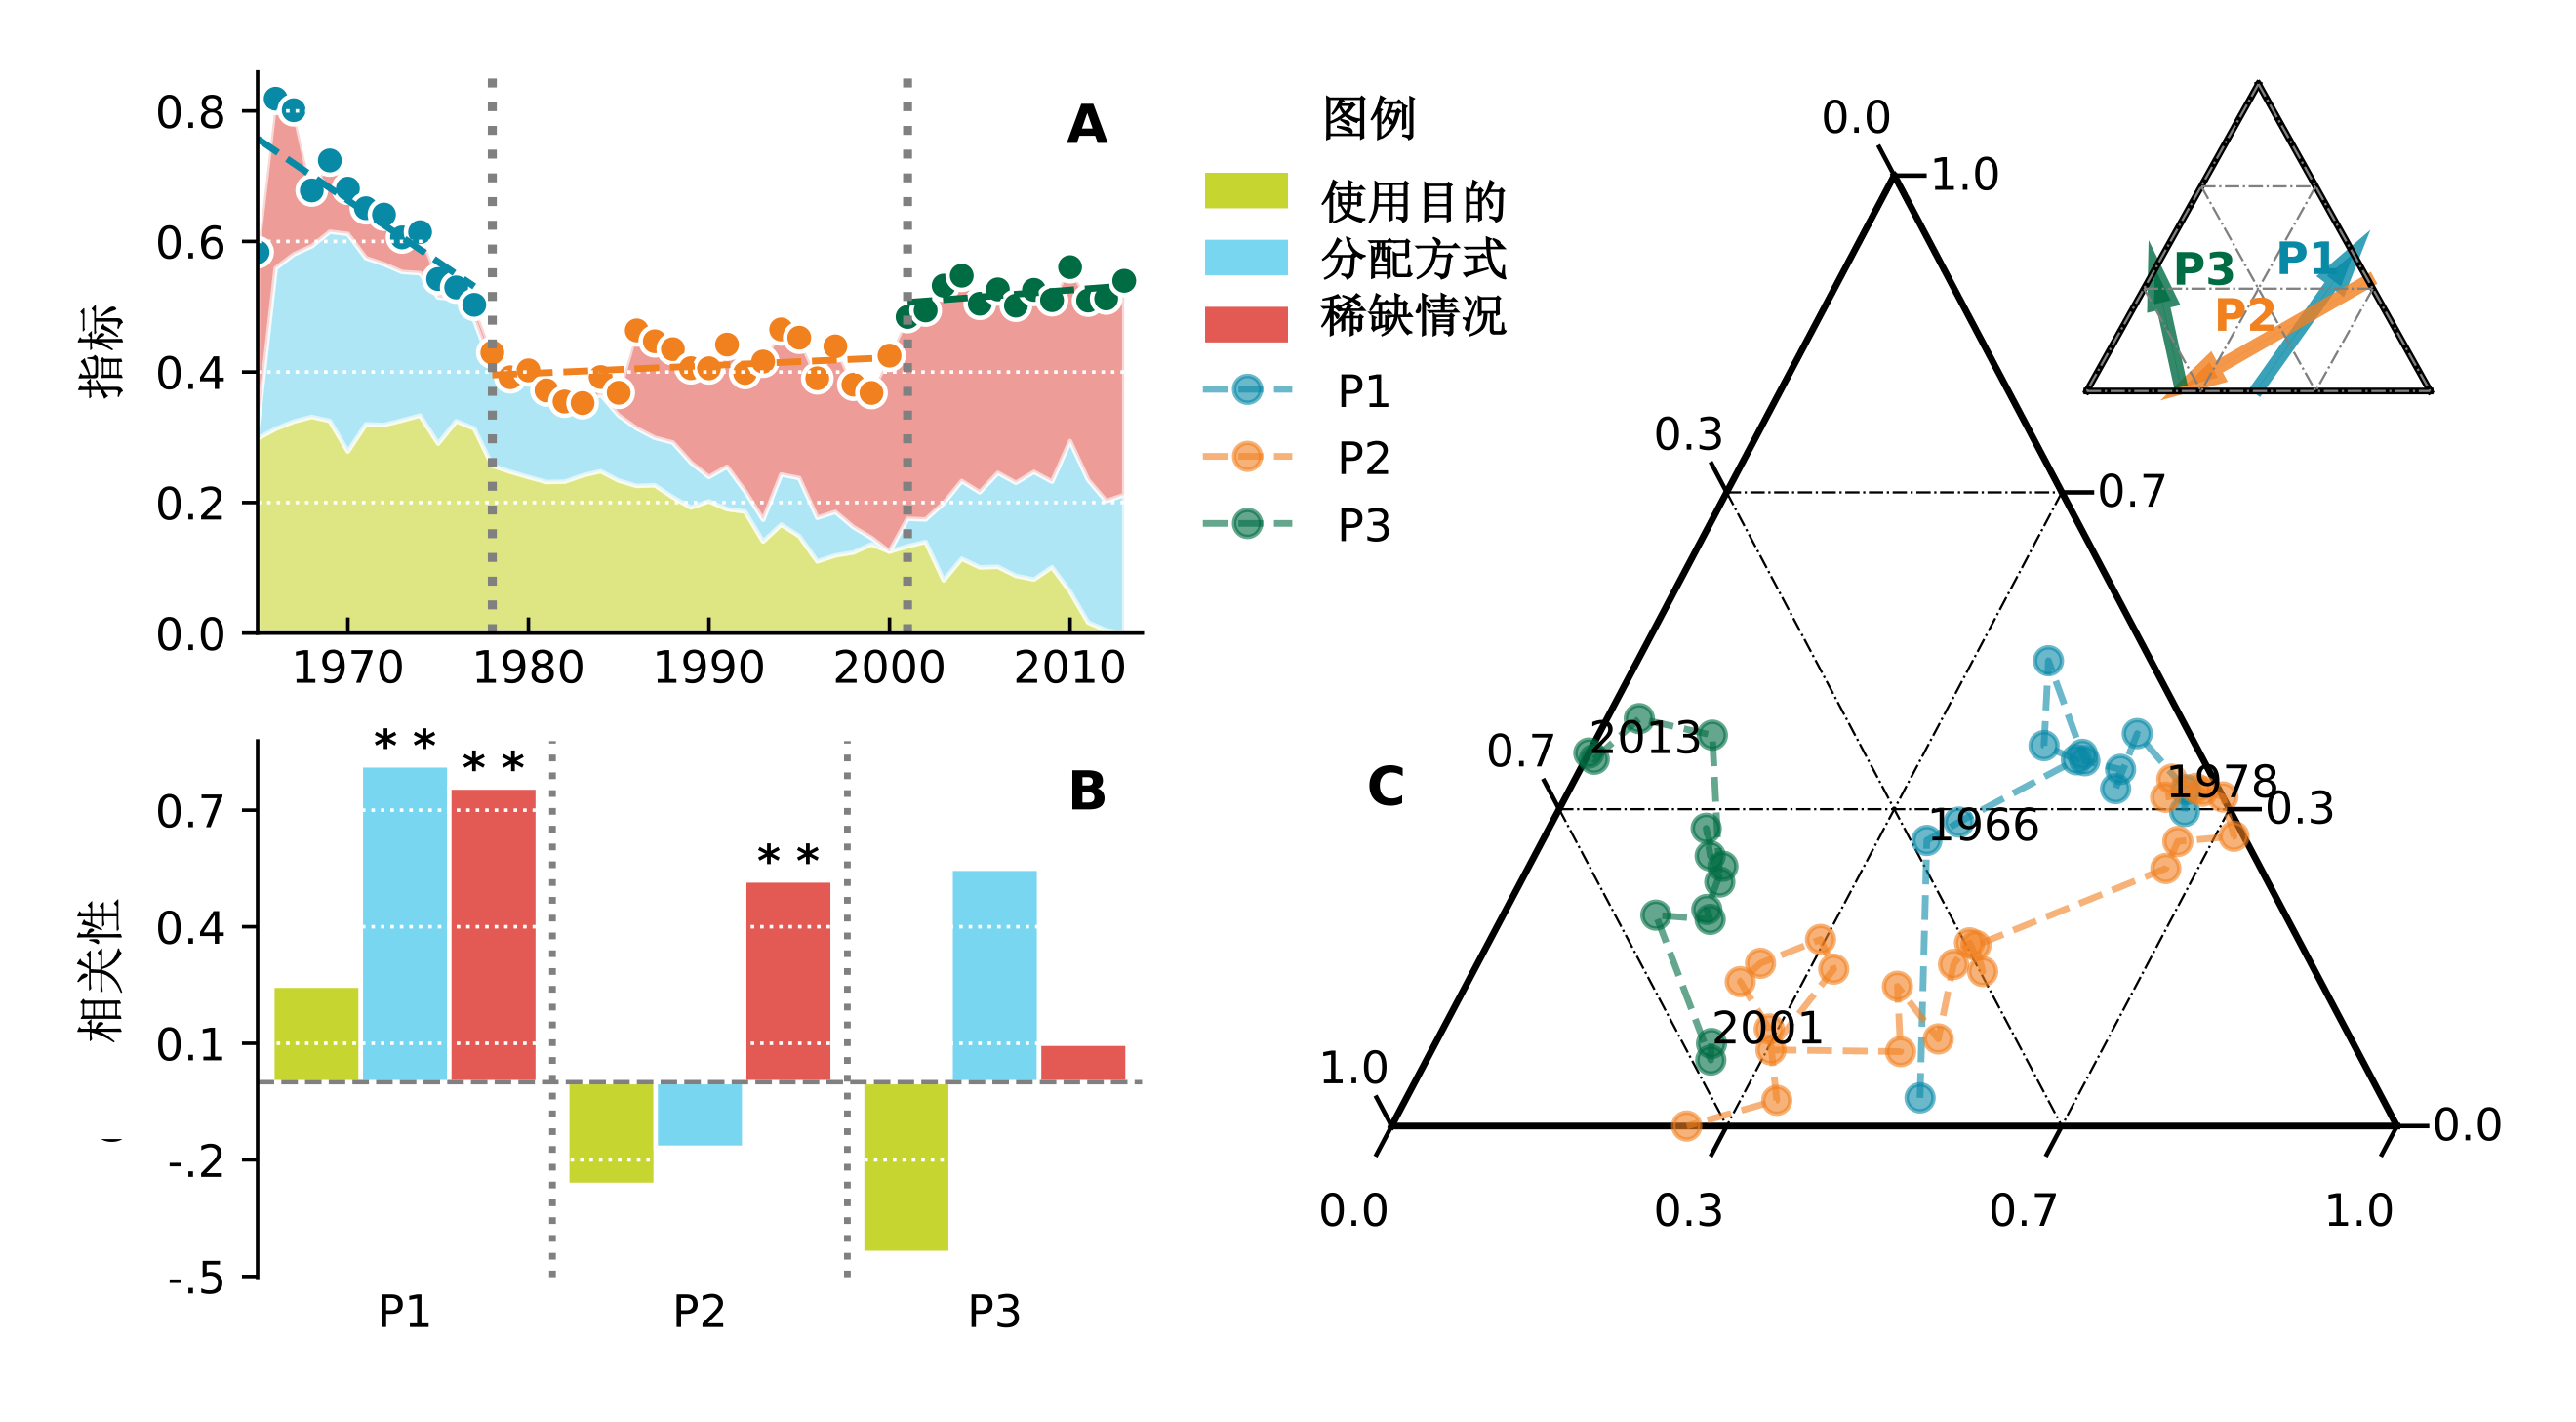
\includegraphics[width=\textwidth]{img/ch4/ch4_index.png}
	\caption[IWGI指数反映黄河流域的水治理变化]{IWGI指数反映黄河流域的水治理变化。两个突变点将1965年以来的黄河流域水治理划分为三个阶段,第一阶段(P1): $1965 \sim 1978$,第二阶段(P2): $1979 \sim 2001$,第三阶段(P3): $2002 \sim 2013$。
	\textbf{A,} 检测IWGI的突变点和三个指标的各自贡献:“多少水(S)”、“怎么用(P)”和“怎么分(A)”。1978年和2001年发生了两个显著的变化点($p<0.01$)。
	\textbf{B,}  各阶段的IWGI变化与三个指标各自变化的相关性。
	\textbf{C,} IWGI随时间变化的同时,三个指标贡献比例的组合不断改变,致使水治理向不同方向发生阶段性转移。
	}\label{ch4:fig:IWGI}
\end{figure*}

两个突变点将1965年以来的黄河流域水治理划分为三个阶段,第一阶段(P1): $1965 \sim 1978$,第二阶段(P2): $1979 \sim 2001$,第三阶段(P3): $2002 \sim 2013$,而“多少水(S)”、“怎么用(P)”和“怎么分(A)”的三个指标在每个阶段做出各自不同的贡献(图~\ref{ch4:fig:IWGI}A)。
% 第一阶段
在第一个时期(P1, $1965 \sim 1978$)水资源压力对IWGI的贡献很小,“怎么用水”和“怎么分水”的指标的贡献大得多(平均分别为$49.45\%$和$34.95\%$),但均呈现出显著的下降趋势($p<0.01$,图~\ref{ch4:fig:IWGI}~B),导致此时期IWGI迅速下降。
% 第二阶段
在第二阶段(P2, $1979 \sim 2001$),水资源压力指标的显著增加($p<0.01$)并一己之力促进了IWGI的略微上升($p<0.01$,图~\ref{ch4:fig:IWGI}~A),而“怎么用水”和“怎么分水”的指标对IWGI的变化起了消极作用。
% 第三阶段
最后,在第三个时期(P3, $1995 \sim 2013$),尽管水资源压力指标在贡献中保持着$57.11\%$的最突出份额,但其数值已几乎保持不变,反而是“怎么用水”的指标的降低和“怎么分水”指标的增加,此消彼长后共同推动了综合指标IWGI的变化。
%的整体
综上所述,“多少水(S)”、“怎么用(P)”和“怎么分(A)”的三个指标在不同时期为黄河流域水治理整体特征的变化做出不同贡献,将其演变历史划分为明显的三个阶段,依据其各自特点可命名为:集中供水时期($1965 \sim 1978$,P1)、治理转型时期($1979 \sim 2001$,P2)、适应增强时期($2002 \sim 2013$,P3)(图~\ref{ch4:fig:IWGI}~C)。
